\documentclass{article}
\usepackage[utf8]{inputenc}

\usepackage{amsmath}
\usepackage{amssymb}
\usepackage{mathtools}
\usepackage[margin=1in]{geometry}
\usepackage{hyperref}
\usepackage{natbib}

\usepackage{tikz}
\usetikzlibrary{quotes}
\usetikzlibrary{bayesnet}
\usetikzlibrary{shapes,arrows}

\title{Routing Games with Drones}
\author{Mark Beliaev}
\date{September, 2022}
\setlength{\parindent}{0pt}
\newcommand{\EX}{\mathbb{E}}
\newcommand{\action}{\mathcal{A}}
\DeclareMathOperator*{\argmax}{arg\,max}
\DeclareMathOperator*{\argmin}{arg\,min}
\definecolor{purple}{rgb}{1, 0, 1}

\newcommand{\ie}{\emph{i.e.,}\xspace}
\newcommand{\eg}{\emph{e.g.,}\xspace}
\newcommand{\abr}{\emph{abbr.}\xspace}
\newcommand{\ea}{\emph{et al.}\xspace}
\newcommand{\gensync}{\emph{GenSync}\xspace}
\newcommand{\colosseum}{\emph{Colosseum}\xspace}
\newcommand{\srep}{\emph{SREP}\xspace} % Set Reconciliation Enhances
\newcommand{\srepsim}{\emph{SREPSim}\xspace}
% Propagation
\newcommand{\esrep}{\emph{E-SREP}\xspace}
\newcommand{\epsrep}{\emph{EP-SREP}\xspace}
\newcommand{\mesrep}{\emph{ME-SREP}\xspace}
\newcommand{\mempoolsync}{\emph{MempoolSync}}

\newcommand{\fref}[1]{Fig.~\ref{#1}}
\newcommand{\tref}[1]{Table~\ref{#1}}
\newcommand{\aref}[1]{Algorithm~\ref{#1}}
\newcommand{\procref}[1]{Procedure~\ref{#1}}
\newcommand{\sref}[1]{Section~\ref{#1}}
\newcommand{\lineref}[1]{line~\ref{#1}}
\newcommand{\appref}[1]{Appendix~\ref{#1}}

% Change \eqref
\LetLtxMacro{\originaleqref}{\eqref}
\renewcommand{\eqref}{Eq.~\originaleqref}

% Theorems and corollaries
\newcounter{theoremcount}
\setcounter{theoremcount}{0}
\DeclareRobustCommand{\theorem}[1]{%
  \refstepcounter{theoremcount}%
  \noindent\textit{\textbf{Theorem \thetheoremcount\label{theorem:#1}: }}%
}
\DeclareRobustCommand{\theoremref}[1]{Theorem~\ref{theorem:#1}}

\DeclareRobustCommand{\proof}{\emph{Proof:}\xspace}
\DeclareRobustCommand{\qqed}{\hfill$\blacksquare$}

\newcounter{corollcount}
\setcounter{corollcount}{0}
\DeclareRobustCommand{\coroll}[1]{%
  \refstepcounter{corollcount}%
  \noindent\textit{\textbf{Corollary \thecorollcount\label{coroll:#1}: }}%
}
\DeclareRobustCommand{\corollref}[1]{Corollary~\ref{coroll:#1}}

\newcounter{lemmacount}
\setcounter{lemmacount}{0}
\DeclareRobustCommand{\lemma}[1]{%
  \refstepcounter{lemmacount}%
  \noindent\textit{\textbf{Lemma \thelemmacount\label{lemma:#1}: }}%
}
\DeclareRobustCommand{\lemmaref}[1]{Lemma~\ref{lemma:#1}}

\newcounter{definitioncount}
\setcounter{definitioncount}{0}
\DeclareRobustCommand{\definition}[1]{%
  \refstepcounter{definitioncount}%
  \noindent\textit{\textbf{Definition \thedefinitioncount\label{definition:#1}: }}%
}
\DeclareRobustCommand{\defref}[1]{Definition~\ref{definition:#1}}

%notes of different authors
\newif\ifnotes
\notestrue
\notesfalse

\newif\ifdiff
\difftrue
\difffalse

\newcommand{\anote}[1]{\ifnotes $\ll$\textsf{\textcolor{purple}{Ari: {#1}}}$\gg$ \fi}
\newcommand{\nnote}[1]{\ifnotes $\ll$\textsf{\textcolor{orange}{Novak: {#1}}}$\gg$ \fi}
\newcommand{\diff}[1]{\ifdiff\textcolor{orange}{#1}\else#1\fi}

%%% Local Variables:
%%% mode: latex
%%% TeX-master: "main"
%%% End:


\begin{document}
	
\maketitle
\section{Introduction}
Our motivation is to look at how delivery operators can adjust prices to optimize for latency and satisfy constraints given a population heterogeneous selfish users. Our end goal is to consider delivery operations that consist of multiple \textit{sources} and \textit{sinks}, each one providing a set of potentially distinct modes of delivery. We abstract this problem by ignoring transportation on networks, instead constructing a bipartite graph between sources and sinks, while treating the edges as delivery options provided to consumers in different areas. We now go over formulations of this problem, starting with the simplest.
	  	
\begin{figure}[!h]
	\centering
	%\resizebox{0.5\textwidth}{!}{%
	\begin{tikzpicture}
	\begin{scope}[->,>=stealth',auto,node distance=3cm,thick,main/.style={circle,draw,font=\sffamily\Large\bfseries,minimum size=1cm}]				
		\node[main] (s) at (0,0) {$s$}; %
		\node[main] (t) at (5,0) {$t$}; %
		
		\draw[->] (s) to [in=160,out=20]   node[font=\sffamily\Large\bfseries,above,align=center]{$\flow_1$} (t);
		\path (s) -- (t) node [font=\Huge, midway, yshift=-.25cm] {$\vdots$};
		\draw[->] (s) to [in=-160,out=-20] node[font=\sffamily\Large\bfseries,below,align=center]{$\flow_\modes$} (t); 
	\end{scope}
	\end{tikzpicture}
	%}%
	\caption{Delivery network with one source $\source$, one sink $\sink$, and $\modes$ edges connecting them.}
	\label{fig:eg1}
\end{figure}
\subsection{Problem}
Let us define the simplest case where our graph $\graph=\{\nodes,\links\}$ consists of one source $\source$ node and one sink $\sink$ node $\nodes=\{\source,\sink\}$, and $\modes$ parallel edges connecting them $\links=\{\link_1,\link_2,\ldots,\link_\modes\}$. We can view the edges $\links$ in our graph $\graph$ as the $\modes$ delivery options provided by the hub $\source$ to users at $\sink$. The amount of deliveries demanded at sink $\sink$ is modeled by an interval $[0,\rate]$ for some constant rate $\rate$. Each point $\user\in[0,\rate]$ is a non-cooperative and infinitesimal unit referred to as a user who decides on which edge to choose. We sort users by money sensitivity, viewing $\pop:[0,\rate]:\rightarrow(0,\infty]$ as a non-decreasing function representing the user's trade-off between price and latency.\par 

We view flow as a Lebesgue-measurable function $\flow:[0,\rate]\rightarrow\links$ which induces a flow over the delivery options provided $\setflow$. Each delivery option has a corresponding continuous, nondecreasing and nonnegative latency function $\latency_i$ that describes the delay experienced by users whose parcels are routed on edge $\link_i$. Additionally, there is a certain cost $\tax_i$ associated with each delivery option $i$ which is controlled to alter the \textit{social cost} experienced by users. Specifically, we let $\cost_{i}^{\user}(\flow,\tax)=\latency_i(\flow_i)+\pop(\user)\tax_i$ represent the cost user $\user\in[0,\rate]$ assigns to delivery option $i$. We call a flow $\nflow$ an equilibrium or Nash flow, if for a certain instance of $(\graph,\pop,\latency,\tax)$, no user $\user\in[0,\rate]$ has incentive to unilaterally alter their strategy by switching from delivery option $\nflow(\user)$ to any $i\in\{1,\ldots,\modes\}$:


\begin{equation}\label{eq:Nash_condition}
	\cost_{\nflow(\user)}^{\user}(\nflow,\tax)\leq \cost_{i}^{\user}(\nflow,\tax).
\end{equation}

In our setting we assume that the delivery hub already has a set of flows $\setflow$ that satisfies the demand $\sum_{i=1}^m=\rate$, and wants to find a set of prices $\settax$ such that the induced equilibrium flow $\nflow$ is equal to the desired flow $\flow$. This means that unlike prior work, we can not rely on the fact that the given $\flow$ minimizes total latency of the graph $\graph$, and instead we want to find prices that could work for any arbitrary flow $\flow$ that satisfies the demand. This is particularly useful when the flow $\flow$ is a solution to an optimization problem with constraints that are not directly imposed on the user equilibrium flows.

\section{Solution}

We know from the more general results of~\cite{roughgarden2003a} that all instances $(\graph,\pop,\latency,\tax)$ admit a flow at Nash equilibrium, and more precisely that one of these Nash flows is canonical: for $\user_1,\user_2\in[0,\rate]$, if $\user_1<\user_2$, then $\latency_{\flow(\user_1)}(\flow)\leq\latency_{\flow(\user_2)}(\flow)$, and if $\user_1>\user_2$, then $\tax_{\flow(\user_1)}\geq\tax_{\flow(\user_2)}(\flow)$. In other words, a canonical Nash flow $\flow$ splits $[0,\rate]$ into a finite number (at most $\modes$) of potentially degenerate sub intervals, inducing an ordering on the paths to which $\flow$ assigns traffic that is non-decreasing in latency and non-increasing in taxes. In addition, all Nash flows induce identical flows on edges if all latency functions are strictly increasing, and $\graph$ is a set of parallel links. Readers can refer to Propositions 2.4 and 2.5 in the referenced paper by~\cite{roughgarden2003a}.\par

The aforementioned properties tell us that for any instance $(\graph,\pop,\latency,\tax)$, there exists a canonical Nash flow $\setnflow$ that sends users in the interval $[\user_{i-1},\user_i]\in[0,\rate]$ on edge $i$ for some corresponding set $\user_0\leq\user_1\leq\ldots\leq\user_\modes$, where $\user_0=0$ and $\user_\modes=\rate$. Say we are given a desired set of flows $\setflow$ sorted in non-decreasing latency: if $i<j$, then $\latency_i\leq\latency_j$ (where the dependency on flow is left out of notation for convenience). Our main result states that any given flow $\setflow$ ordered by non-decreasing latency is an equilibrium flow for instance $(\graph,\pop,\latency,\tax)$ where $\pop(0)>0$ (\textit{may not be needed}), and for any $\tax_\modes$:

\begin{equation}\label{eq:main_result_recursive}
	\tax_i=\tax_{i+1}+\frac{\latency_{i+1}-\latency_{i}}{\pop(\user_i)} \qquad\forall i\in\{1,\ldots,\modes-1\}.
\end{equation}

Simplifying the recursion above yields:

\begin{equation}\label{eq:main_result}
	\tax_i=\tax_\modes+\sum_{k=i}^{m-1}\frac{\latency_{k+1}-\latency_{k}}{\pop(\user_k)} \qquad\forall i\in\{1,\ldots,\modes-1\}.
\end{equation}

Note that although the equations above hold for any fare $\tax_\modes$, since $\tax_\modes$ corresponds to the road with the lowest tax and most price averse users, one can simply set $\tax_\modes=0$. 

\section{Proof}
The proof is as follows: using a subset of the inequalities defined for Nash equilibrium in Eq.~\eqref{eq:Nash_condition}, we first show that for some desired Nash flow $\flow$ there is only one set of valid taxes $\tax$ that satisfy this subset of inequalities. We complete the proof by showing that the corresponding set of taxes $\tax$ does indeed satisfy all of the inequalities defined in Eq.~\eqref{eq:Nash_condition}. 

\begin{figure}[!h]
	\centering
	\begin{tikzpicture}[scale=7]
		\draw[-, thick] (0,0) -- (1,0);
		\foreach \x/\xtext in {0/0,0.3/$\user_{i-1}$,0.5/$\user_{i}$,0.7/$\user_{i+1}$,1/$\rate$}
		\draw[thick] (\x,0.5pt) -- (\x,-0.5pt) node[below] {\xtext};
		\draw (0.15,-1pt) node {$\ldots$};
		\draw (0.85,-1pt) node {$\ldots$};
		\draw[[-), ultra thick, blue] (0.3,0) -- (0.5,0);
		\draw[[-), ultra thick, red] (0.5,0) -- (0.7,0);
		\draw (-0.36,1pt) node {$\user\in[\user_0,\user_\modes], \user_0=0, \user_\modes=\rate$};
		\draw (-0.4,-1pt) node {$\forall \user\in [\user_{i-1},\user_i): \flow(\user)=i $};
		\draw (0.4,3pt) node {$\tax_i$};
		\draw (0.4,1.5pt) node {$\latency_i$};
		\draw (0.6,3pt) node {$\tax_{i+1}$};
		\draw (0.6,1.5pt) node {$\latency_{i+1}$};
		\draw (0.5,3pt) node {$\geq$};
		\draw (0.5,1.5pt) node {$\leq$};
		%\draw (0.4,-1.5pt) node {$\flow_i$};
		%\draw (0.6,-1.5pt) node {$\flow_{i+1}$};
	\end{tikzpicture}
	\caption{Intervals}
	\label{fig:proof intervals}
\end{figure}

We define two adjacent intervals that are formed by our flow $\flow$: users $\user\in[\user_{i-1},\user_i]$ on the left are on $\link_i$ with latency $\latency_i(\flow_i)$ and tax $\tax_i$, while users $\user\in[\user_{i},\user_{i+1}]$ on the right are on $\link_{i+1}$ with latency $\latency_{i+1}(\flow_{i+1})$ and tax $\tax_{i+1}$. The two intervals are portrayed in Fig.~\ref{fig:proof intervals}, where we note that this definition holds for $i=\{1,\ldots,\modes-1\}$. Using the inequalities defined in Eq.~\eqref{eq:Nash_condition}, we know that for $\flow$ to be a Nash flow for instance $(\graph,\pop,\latency,\tax)$, no user $\user$ from the left interval $\user\in[\user_{i-1},\user_i]$ traveling on edge $\link_i$ should want to switch to $\link_{i+1}$ on the right:

\begin{equation}\label{eq:left_to_right}
	\latency_i+\pop(\user)\tax_i \leq \latency_{i+1}+\pop(\user)\tax_{i+1} \quad\forall\user\in[\user_{i-1},\user_i],
\end{equation}
where we leave out denoting the flow $\flow_i$ in latency function $\latency_i(\flow_i)$. It follows:

\begin{align}
	\latency_i+\pop(\user)\tax_i &\leq \latency_{i+1}+\pop(\user)\tax_{i+1} \quad\forall\user\in[\user_{i-1},\user_i],\\
	\tax_i -\tax_{i+1} &\leq \frac{\latency_{i+1}-\latency_{i}}{\pop(\user)} \quad\forall\user\in[\user_{i-1},\user_i],\\
	\tax_i -\tax_{i+1} &\leq \min_{\user\in[\user_{i-1},\user_i]}\Big({\frac{\latency_{i+1}-\latency_{i}}{\pop(\user)}}\Big).
\end{align}

The preceding inequality can be simplified further by using the non-decreasing property of function $\pop$ defining the population's price sensitivity: for any $\user_1,\user_2\in[0,\rate]$ such that $\user_1\leq\user_2$, given user $\user\in[\user_1,\user_2]$, $\max{\pop(\user)}=\pop(\user_2)$ and $\min{\pop(\user)}=\pop(\user_1)$. This comparison results in the following condition which must be true for $\flow$ to be a Nash flow:   
\begin{equation}\label{eq:left_ineq}
	\tax_i -\tax_{i+1} \leq {\frac{\latency_{i+1}-\latency_{i}}{\pop(\user_i)}}.
\end{equation}

We can repeat this process by enforcing that no user $\user$ from the right interval $\user\in[\user_{i},\user_{i+1}]$ traveling on $\link_{i+1}$ should want to switch to edge $\link_i$ on the left:

\begin{align}
	\latency_{i+1}+\pop(\user)\tax_{i+1} &\leq \latency_{i}+\pop(\user)\tax_{i} \quad\forall\user\in[\user_{i},\user_{i+1}],\\
	\tax_i -\tax_{i+1} &\geq \frac{\latency_{i+1}-\latency_{i}}{\pop(\user)} \quad\forall\user\in[\user_{i},\user_{i+1}],\\
	\tax_i -\tax_{i+1} &\geq \max_{\user\in[\user_{i},\user_{i+1}]}\Big({\frac{\latency_{i+1}-\latency_{i}}{\pop(\user)}}\Big),
\end{align}
	which results in the following:

\begin{equation}\label{eq:right_ineq}
	\tax_i -\tax_{i+1} \geq {\frac{\latency_{i+1}-\latency_{i}}{\pop(\user_i)}}.
\end{equation}

From \eqref{eq:left_ineq} and \eqref{eq:right_ineq} we can see that the two inequalities force the set of taxes $\settax$ to follow:
\begin{equation}\label{eq:proof_eq}
	\tax_i -\tax_{i+1} = {\frac{\latency_{i+1}-\latency_{i}}{\pop(\user_i)}} \quad\forall i\in\{1,\ldots,\modes-1\},
\end{equation}
where if $\tax_\modes$ is given, the rest of the prices can be found recursively as defined in Eqs. \eqref{eq:main_result_recursive} and \eqref{eq:main_result}:
\begin{equation}\label{eq:main_result_repeated}
	\tax_i=\tax_\modes+\sum_{k=i}^{m-1}\frac{\latency_{k+1}-\latency_{k}}{\pop(\user_k)} \qquad\forall i\in\{1,\ldots,\modes-1\}.
\end{equation}
To complete the proof, we must show that for this set of taxes $\tax$, the desired $\flow$ is indeed an equilibrium flow. Formally, $\flow$ is an equilibrium flow for instance $(\graph,\pop,\latency,\tax)$ if for all edges $i\in\{1,\ldots,\modes\}$ no user $\user$ in interval $\user\in[\user_{i-1},\user_i]$ should want to switch to any other edge $j\in\{1,\ldots,\modes\}$:
\begin{equation}\label{eq:proof_all_ineq}
	\latency_i+\pop(\user)\tax_i \leq \latency_{j}+\pop(\user)\tax_{j} \quad\forall\user\in[\user_{i-1},\user_i],\forall i\in\{1,\ldots,\modes\},\forall j\in\{1,\ldots,\modes\}.
\end{equation}
Clearly these inequalities hold when $i=j$, and hence we show that they hold when $i>j$ and $i<j$. Starting with the former, when $i>j$ we are considering that no user on edge $\link_i$ will switch to any edge $\link_j$ on the left, where by definition $\tax_i\leq\tax_j$ and $\latency_i\geq\latency_j$. Rearranging Eq.~\ref{eq:proof_all_ineq}, we have:
\begin{align}
	\latency_i+\pop(\user)\tax_i &\leq \latency_j+\pop(\user)\tax_{j} \quad\forall\user\in[\user_{i-1},\user_i],\forall i>j,\\
	\tax_j -\tax_i &\geq \max_{\user\in[\user_{i-1},\user_{i}]}\Big(\frac{\latency_i-\latency_j}{\pop(\user)}\Big) \quad\forall i>j,\\
	\tax_\modes+\sum_{k=j}^{m-1}\frac{\latency_{k+1}-\latency_{k}}{\pop(\user_k)} - \tax_\modes-\sum_{k=i}^{m-1}\frac{\latency_{k+1}-\latency_{k}}{\pop(\user_k)}&\geq \frac{\latency_i-\latency_j}{\pop(\user_{i-1})} \quad\forall i>j,\\
	\sum_{k=j}^{i-1}\frac{\latency_{k+1}-\latency_{k}}{\pop(\user_k)}&\geq \sum_{k=j}^{i-1}\frac{\latency_{k+1}-\latency_{k}}{\pop(\user_{i-1})} \quad\forall i>j.
\end{align}
Since $\pop(\user_{i-1})\geq\pop(\user_k)$ when $j\leq k \leq i-1$, every summation term on the left hand side is strictly greater than or equal to every summation term on the right hand side, validating the inequalities in Eq.~\ref{eq:proof_all_ineq} for $i>j$. We can do the same for $i<j$, where now $\tax_i\geq\tax_j$ and $\latency_i\leq\latency_j$:
\begin{align}
	\latency_i+\pop(\user)\tax_i &\leq \latency_j+\pop(\user)\tax_{j} \quad\forall\user\in[\user_{i-1},\user_i],\forall i<j,\\
	\tax_i -\tax_j &\leq \min_{\user\in[\user_{i-1},\user_{i}]}\Big(\frac{\latency_j-\latency_i}{\pop(\user)}\Big) \quad\forall i<j,\\
	\tax_\modes+\sum_{k=i}^{m-1}\frac{\latency_{k+1}-\latency_{k}}{\pop(\user_k)} - \tax_\modes-\sum_{k=j}^{m-1}\frac{\latency_{k+1}-\latency_{k}}{\pop(\user_k)}&\leq \frac{\latency_i-\latency_j}{\pop(\user_{i})} \quad\forall i<j,\\
	\sum_{k=i}^{j-1}\frac{\latency_{k+1}-\latency_{k}}{\pop(\user_k)}&\leq \sum_{k=i}^{j-1}\frac{\latency_{k+1}-\latency_{k}}{\pop(\user_{i})} \quad\forall i<j.
\end{align}
This time, since $\pop(\user_{i})\leq\pop(\user_k)$ when $i\leq k \leq j-1$, every summation term on the left hand side is strictly less than or equal to every summation term on the right hand side. This completes the proof.

\bibliographystyle{unsrtnat}
\bibliography{refs.bib}
\end{document}
\section{Extension}
\begin{figure}[!h]
	\centering
	%\resizebox{0.5\textwidth}{!}{%
	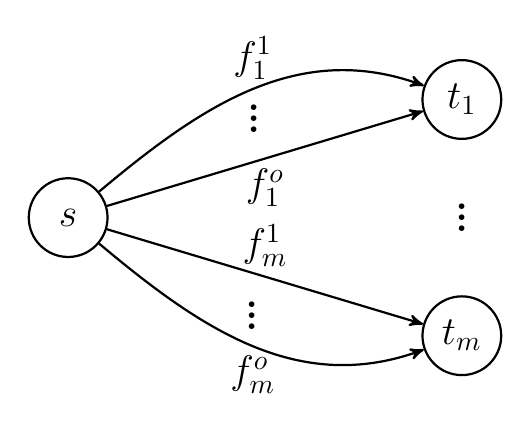
\begin{tikzpicture}
	\begin{scope}[->,>=stealth',auto,node distance=3cm,thick,main/.style={circle,draw,font=\sffamily\Large\bfseries,minimum size=1cm}]				
		\node[main] (s)   at (0,0)  {$s$}; %
		\node[main] (t1)  at (5,1.5)  {$t_1$}; %
		\node[font=\Huge, yshift=.1cm] at (5,0)  {$\vdots$}; %
		\node[main] (tm)  at (5,-1.5) {$t_m$}; %

		\draw[->] (s) to [in=160,out=40] node[font=\sffamily\Large\bfseries,above,align=center]{$f^1_1$} (t1);
		\path (s) -- (t1) node[font=\Huge, midway, yshift=.2cm, xshift=.1cm] {$\vdots$};
		\draw[->] (s) to node[font=\sffamily\Large\bfseries,below,align=center]{$f^o_1$} (t1); 
		
		\draw[->] (s) to  node[font=\sffamily\Large\bfseries,above,align=center]{$f^1_m$} (tm);
		\path (s) -- (tm) node [font=\Huge, midway, yshift=-.8cm, xshift=-.4cm] {$\vdots$};
		\draw[->] (s) to [in=-160,out=-40] node[font=\sffamily\Large\bfseries,below,align=center]{$f^o_m$} (tm); 
	\end{scope}
	\end{tikzpicture}
		%}%
	\caption{Delivery network with one source $s$ and $m$ sinks $t_k$ for $k\in[m]$.}
	\label{fig:eg2}
\end{figure}


		
